\documentclass{beamer}
\usepackage[utf8]{inputenc}

\usetheme{Madrid}
\usecolortheme{default}
\usepackage{amsmath,amssymb,amsfonts,amsthm}
\usepackage{txfonts}
\usepackage{tkz-euclide}
\usepackage{listings}
\usepackage{adjustbox}
\usepackage{array}
\usepackage{tabularx}
\usepackage{gvv}
\usepackage{lmodern}
\usepackage{circuitikz}
\usepackage{tikz}
\usepackage{graphicx}

\setbeamertemplate{page number in head/foot}[totalframenumber]

\usepackage{tcolorbox}
\tcbuselibrary{minted,breakable,xparse,skins}



\definecolor{bg}{gray}{0.95}
\DeclareTCBListing{mintedbox}{O{}m!O{}}{%
  breakable=true,
  listing engine=minted,
  listing only,
  minted language=#2,
  minted style=default,
  minted options={%
    linenos,
    gobble=0,
    breaklines=true,
    breakafter=,,
    fontsize=\small,
    numbersep=8pt,
    #1},
  boxsep=0pt,
  left skip=0pt,
  right skip=0pt,
  left=25pt,
  right=0pt,
  top=3pt,
  bottom=3pt,
  arc=5pt,
  leftrule=0pt,
  rightrule=0pt,
  bottomrule=2pt,
  toprule=2pt,
  colback=bg,
  colframe=orange!70,
  enhanced,
  overlay={%
    \begin{tcbclipinterior}
    \fill[orange!20!white] (frame.south west) rectangle ([xshift=20pt]frame.north west);
    \end{tcbclipinterior}},
  #3,
}
\lstset{
    language=C,
    basicstyle=\ttfamily\small,
    keywordstyle=\color{blue},
    stringstyle=\color{orange},
    commentstyle=\color{green!60!black},
    numbers=left,
    numberstyle=\tiny\color{gray},
    breaklines=true,
    showstringspaces=false,
}
%------------------------------------------------------------
%This block of code defines the information to appear in the
%Title page
\title %optional
{2.8.10}
\date{September 6,2025}


\author 
{Jnanesh Sathisha karmar - EE25BTECH11029}



\begin{document}



\frame{\titlepage}
\begin{frame}{Question}
If with reference to the right handed system of mutually perpendicular unit vectors
$\hat{i},\hat{j}$ and $\hat{k}, \vec{\alpha} = 3\hat{i}-\hat{j},\vec{\beta} = 2\hat{i} +\hat{j} - 3\hat{k},$ then express $\beta$ in the form $\beta =\beta_1 +\beta_2$ where $\beta_1$ is parallel to $\alpha$ and $\beta_2$ is perpendicular to $\alpha$
\end{frame}



\begin{frame}{Equation}
Given details:
\begin{align}
    \vec{\alpha} &= 3\hat{i}-\hat{j}=\myvec{3 \\ -1\\0}\\\vec{\beta} &= 2\hat{i} +\hat{j} - 3\hat{k}=\myvec{2\\1\\-3}
\end{align}
\end{frame}
\begin{frame}{Theoretical Solution}

$\beta_1$ is a projection of $\beta$ on $\alpha$\\
The projection formula for projection is: 
\begin{align}
\beta_1&=\frac{\vec{\beta^T}\vec{\alpha}}{\norm{\vec{\alpha^2}}}\vec{\alpha}
\end{align}
\end{frame}

\begin{frame}{Theoretical Solution}
\begin{align}
&=\frac{\myvec{2&&1&&-3}\myvec{3\\-1\\0}}{\brak{3}^2+\brak{-1}^2+\brak{0}^2}\myvec{3\\-1\\0}\\
&=\frac{5}{10}\myvec{3\\-1\\0}\\
&=\myvec{\frac{3}{2}\\ \frac{-1}{2}\\ 0}
\end{align}
\end{frame}


\begin{frame}{Theoretical Solution}
Now according to the given equation :
\begin{align}
    \beta&=\beta_1+\beta_2\\
    \beta_2&=\beta-\beta_1\\
    \beta_2&=\myvec{2\\1\\-3}-\myvec{\frac{3}{2}\\ \frac{-1}{2}\\0}\\
    \beta_2&=\myvec{\frac{1}{2}\\ \frac{3}{2}\\-3}
\end{align}
\end{frame}
\begin{frame}{Theoretical Solution}
Lets verify wheter $\beta_2$ is perpendicular to $\alpha$\\
For that:
\begin{align}
    \alpha^T.\beta_2&=0\\
    \myvec{3&&-1&&0}\myvec{\frac{1}{2}\\ \frac{3}{2}\\-3}&=\myvec{0}
\end{align}
Therefore $\beta_2$ is perpendicular to $\alpha$
\end{frame}
\begin{frame}{Theoretical Solution}
Therefore $\beta$ is:
\begin{align}
    \beta&=\beta_1+\beta_2\\
    \beta&=\myvec{\frac{3}{2}\\ \frac{-1}{2}\\0}+\myvec{\frac{1}{2}\\ \frac{3}{2}\\-3}
\end{align}
\end{frame}

\begin{frame}[fragile]
    \frametitle{C Code (1) - Function to store the points }

    \begin{lstlisting}

#include <stdio.h>
 
double start_points[4][3]={
	{0.0,0.0,0.0},
	{0.0,0.0,0.0},
	{0.0,0.0,0.0},
	{0.0,0.0,0.0}
};
double end_points[4][3]={
	{3.0,-1.0,0.0},
	{2.0,1.0,-3.0},
	{3/2,-1/2,0.0},
	{1/2,3/2,-3.0}



    \end{lstlisting}
\end{frame}
\begin{frame}[fragile]
    \frametitle{C Code (1) - Function to store the points }

    \begin{lstlisting}
};
void get_start_points(double *arr){
	for (int i=0;i<4;i++){
		arr[i*3+0]=start_points[i][0];
		arr[i*3+1]=start_points[i][1];
		arr[i*3+2]=start_points[i][2];
	}
}
void get_end_points(double *arr){
	for (int i=0;i<4;i++){
		arr[i*3+0]=end_points[i][0];
		arr[i*3+1]=end_points[i][1];
		arr[i*3+2]=end_points[i][2];
	}
}
 \end{lstlisting}
\end{frame}

\begin{frame}[fragile]
    \frametitle{Python Code - Using Shared Object}
    \begin{lstlisting}

import ctypes
import numpy as np
import matplotlib.pyplot as plt
import subprocess
y=input("are you using termux?(y/n)=")


lib = ctypes.CDLL('./vectors.so')

lib.get_start_points.argtypes = [ctypes.POINTER(ctypes.c_double)]
lib.get_end_points.argtypes = [ctypes.POINTER(ctypes.c_double)]



\end{lstlisting}
\end{frame}

\begin{frame}[fragile]
    \frametitle{Python Code - Using Shared Object}
    \begin{lstlisting}
n_lines = 4

start_points = np.zeros((n_lines,3), dtype=np.float64)
end_points   = np.zeros((n_lines,3), dtype=np.float64)
lib.get_start_points(start_points.ctypes.data_as(ctypes.POINTER(ctypes.c_double)))
lib.get_end_points(end_points.ctypes.data_as(ctypes.POINTER(ctypes.c_double)))


fig = plt.figure()
ax = fig.add_subplot(111, projection='3d')

colors = ['r','g','b','m']
label=['alpha','beta','beta1','beta2']

\end{lstlisting}
\end{frame}
\begin{frame}[fragile]
    \frametitle{Python Code - Using Shared Object}
    \begin{lstlisting}
for i in range(n_lines):
    xs = [start_points[i,0], end_points[i,0]]
    ys = [start_points[i,1], end_points[i,1]]
    zs = [start_points[i,2], end_points[i,2]]
    ax.plot(xs, ys, zs, color=colors[i], label=label[i])

ax.set_xlabel('X')
ax.set_ylabel('Y')
ax.set_zlabel('Z')
ax.legend()
plt.title("3D Lines from C Library")
fig.savefig('../figs/fig2.png')
if (y=='y'):
    subprocess.run(shlex.split('termux-open ../figs/fig.png'))
else:
    subprocess.run(["open",  "../figs/fig.png"])
plt.show()





\end{lstlisting}
\end{frame}



\begin{frame}{Plot-Using Both C and Python}
    \centering
    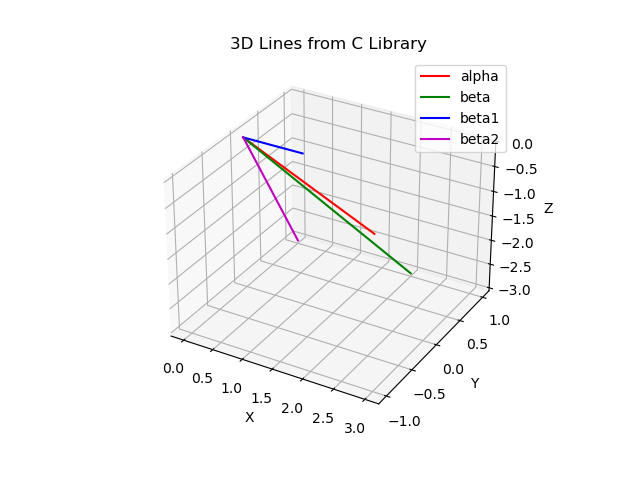
\includegraphics[width=\columnwidth, height=0.8\textheight, keepaspectratio]{figs/fig2.png}     
\end{frame}

\begin{frame}[fragile]
    \frametitle{Python Code}
    \begin{lstlisting}
import numpy as np
import matplotlib.pyplot as plt
import sys
import subprocess
print('Using termux?(y/n)')
y = input()
alpha=np.array([3,-1,0])
beta=np.array([2,1,-3])
beta1=np.array([3/2,-1/2,0])
beta2=np.array([1/2,3/2,-3])







\end{lstlisting}
\end{frame}

\begin{frame}[fragile]
    \frametitle{Python Code }
    \begin{lstlisting}
fig=plt.figure()
ax=fig.add_subplot(111,projection='3d')
ax.plot([0,alpha[0]],[0,alpha[1]],[0,alpha[2]],'b-',label='alpha')
ax.plot([0,beta[0]],[0,beta[1]],[0,beta[2]],'g-',label='beta')
ax.plot([0,beta1[0]],[0,beta1[1]],[0,beta1[2]],'r-',label='beta1')
ax.plot([0,beta2[0]],[0,beta2[1]],[0,beta2[2]],color='pink',label='beta')



\end{lstlisting}
\end{frame}
\begin{frame}[fragile]
    \frametitle{Python Code }
    \begin{lstlisting}
ax.set_xlabel('$x$')
ax.set_ylabel('$y$')
ax.set_zlabel('$z$')
ax.legend(loc='best')
ax.grid(True)
ax.axis('equal')
fig.savefig('../figs/fig.png')
print('Saved figure to ../figs/fig.png')

if(y == 'y'):
    subprocess.run(shlex.split('termux-open ../figs/fig.png'))
else:
    subprocess.run(["open",  "../figs/fig.png"])
 
plt.show()
\end{lstlisting}
\end{frame}




\begin{frame}{Plot-Using only Python}
    \centering
    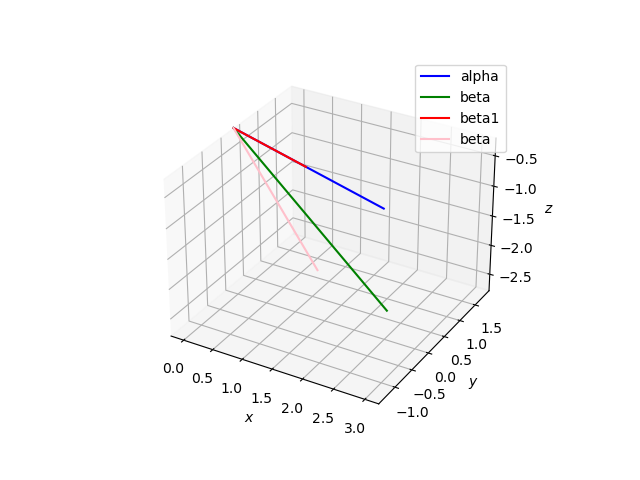
\includegraphics[width=\columnwidth, height=0.8\textheight, keepaspectratio]{figs/fig.png}     
\end{frame}


\end{document}